\documentclass[]{article}

\usepackage{geometry}
\usepackage{amsmath}
\usepackage{authblk}
\usepackage{graphicx}
\usepackage{subcaption}
%\geometry{
%	a4paper,
%	total={170mm,257mm},
%	left=20mm,
%	top=20mm,
%}

%opening
\title{Plant recommendation using environment and biotic associations - GeoLifeCLEF 2019 Working Notes}
%\title{Distributed representations for location-based species recommendation}
%\title{Distributed representations of species niches for location-based recommendation}
%\title{Deep plant recommendation using environment and biotic associations}
%\title{Contrasting Grinnellian and Eltonian niche concepts for geographic species recommendation}
%\title{Ecological niche concepts for geographic species recommendation}
%\title{Deep learning local dominant plant species given environment and biotic associations}
%\title{Embedding grinnellian and eltonian niches for location-based plant recommendation}
%\title{Embedding grinnellian and eltonian niches for geographic plant recommendation}

\author[1,2,3]{Sara Si-Moussi}
\author[2]{Esther Galbrun}
\author[1]{Mickael Hedde}
\author[1]{Tanguy Daufresne}
\author[3]{Wilfried Thuiller}

\affil[1]{Eco\&Sols, UMR 1222 INRA-Montpellier SupAgro, Montpellier}
\affil[2]{Loria, UMR 7503 Inria, Vandœuvre-lès-Nancy}
\affil[3]{LECA, UMR 5553 CNRS-Université Grenoble Alpes, Saint-Martin-d'Hères}
\date{}                     %% if you don't need date to appear
\setcounter{Maxaffil}{0}
\renewcommand\Affilfont{\itshape\small}

\graphicspath{ {./figures/} }
\begin{document}
	
	\maketitle

\begin{abstract}
	\noindent Automatically predicting species composition in geographic locations is of great importance for biodiversity conversation. Inspired by ecological concepts of Grinnellian and Eltonian niche, we investigate two neural network architectures that attempt to extract these niches' features for plant recommendation.  The first proposal uses environmental rasters and leverages advanced feature extraction techniques based on distributed representations and convolutional neural networks. The second proposal relies on neighboring co-occurrences with organisms from an expert-curated list of taxa. We find that the former solution outperforms the latter in prediction accuracy, yet the second solution provides interesting and more interpretable indicators. Both approaches yielded promising results on the GeoLifeCLEF 2019 challenge. \\
	
	\noindent \textbf{Keywords}: Distributed representations, Convolutional Neural Networks, Species Distribution Models, Ecological niche theory, Plant ecology
\end{abstract}


\section{Introduction}
Predicting the most likely species in a given location is of great importance in biodiversity studies. This age-old question in biogeography is commonly solved through Species Distribution Modeling (SDM) or Habitat Suitability Modeling (HSM). The task consists in learning a density function of the species over the geographic space from a set of observed geolocalized occurrences. In practice, due to sampling bias, limited examples and local habitat heterogeneity, geographic coordinates are not used directly as predictors. Instead, SDMs predict species abundance as a function of the environmental conditions at the given locations.\\

\noindent The local environment is usually described by abiotic features such as climate and pedology. Recently, more studies include biotic covariates in the form of other living beings abundance. The latter use is motivated by the need to account for the dependencies between species that can affect their co-distributions. Indeed, two species distributions may be correlated indirectly through a latent abiotic variable or directly if they interact in some way that creates a dependency between their respective populations as in the case of plant-pollinators, host-parasites, predator-preys, etc.\\

\noindent The set of locations with suitable abiotic conditions for a given species define its \textit{Grinnellian niche}\cite{grinnell1917niche}. On the other hand, the role it occupies within its community through feeding on other organisms or interacting with them defines its \textit{Eltonian niche}\cite{elton2001animal} or its biotic requirements. The intersection of the sets of locations falling within both niches produces the species \textit{Fundamental niche}. What we observe is an accessible subset of it called the \textit{Realized niche} \cite{peterson2011ecological}. \\
 
\noindent In the context of GeoLifeCLEF 2019 challenge, we evaluate two models on location-based plant recommendation. The first one relies purely on abiotic features while the second makes use of regional level co-occurrences with other organisms curated with expert assistance. We describe both solutions and discuss results obtained during training, validation and test phases.  %Un peu plus d'infos sur la task%


\section{Dataset description}
Task organizers provided a training dataset containing about 280K observations from the Global Biodiversity and Information Facility database. Additionally, nearly 2M plant occurrences from automatic species identification of pictures produced in 2017--2018 by the smartphone application Pl@ntNet were added. We used the complete plant occurrences involving almost 3.5K plant taxa. Besides, 10M occurrences from other biodiversity kingdoms were also included. Finally, 33 environmental rasters covering the French territory were provided. They describe the climate, topology and pedological landscape. They were constructed from various open datasets as explained in the protocol note. %Output attendu%


\section{Task and proposals}
The task consists on training a model that predicts at a geographic point the dominant plant species. We solve for a multi-class classification problem where the output class is the dominant plant identity. We evaluate two architectures for solving the task:
\begin{itemize}
	\item \textit{GrinnellNet}: A convolutional neural network architecture using environmental rasters. It supposedly learns features of species Grinnellian niche.
	\item \textit{EltonNet}: A species embedding network leveraging associations with nearest non-plant taxa occurrences. Its purpose is to identify community composition patterns that are positively associated to plant species, possibly related to the Eltonian niche concept.
\end{itemize}

\noindent Hereafter, we describe both proposals and motivate our architecture, preprocessing and optimization choices.

\subsection{GrinnellNet: a CNN with categorical rasters embedding}
GrinnellNet's architecture (illustrated in Figure \ref{grinnellnet}) is organized in a stack of components trained end-to-end: input preprocessing, feature extraction, feature interaction and classification. It takes environmental rasters as inputs and returns the identity of the dominant plants. We refer to the latter with the term \textbf{class} in this report.

\begin{figure}
	\begin{subfigure}{0.5\textwidth}
		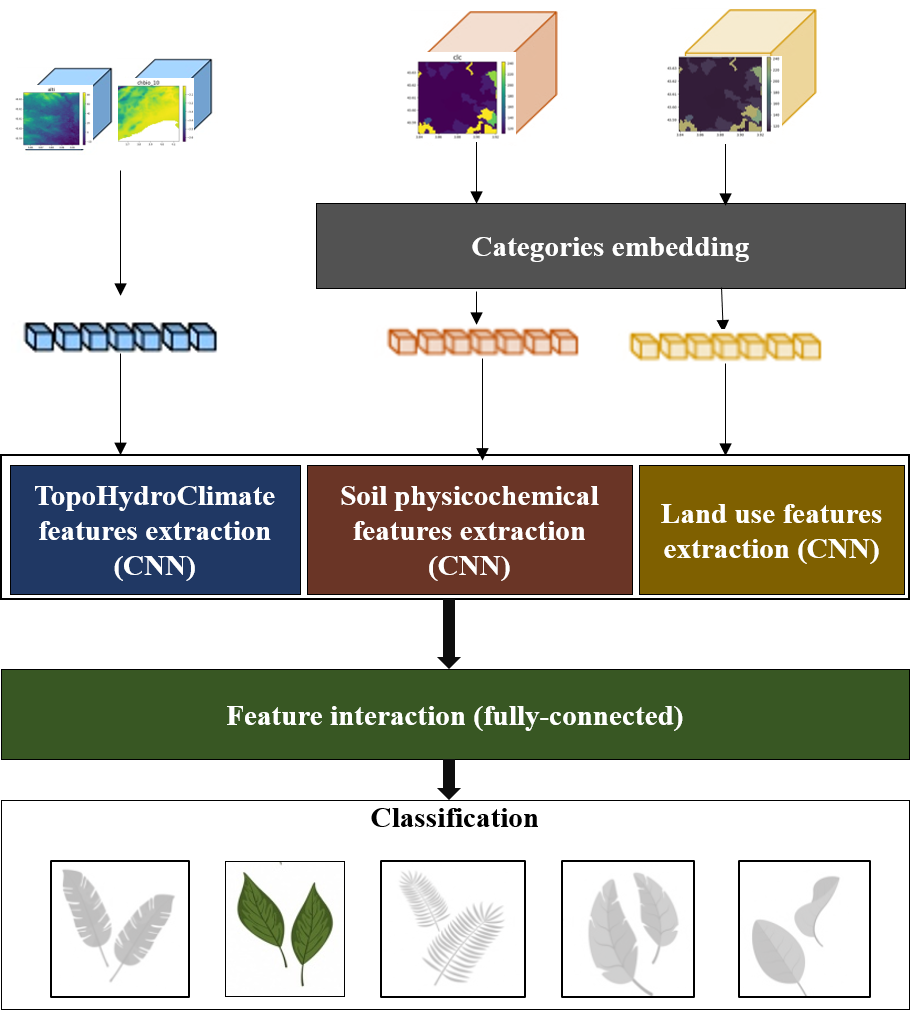
\includegraphics[scale=0.4]{grinnellsep.png}
		\caption{SepGrinnellNet: separate feature extraction modules} \label{grinnellnet:a}
	\end{subfigure}
	\hspace*{\fill} % separation between the subfigures
	\begin{subfigure}{0.5\textwidth}
		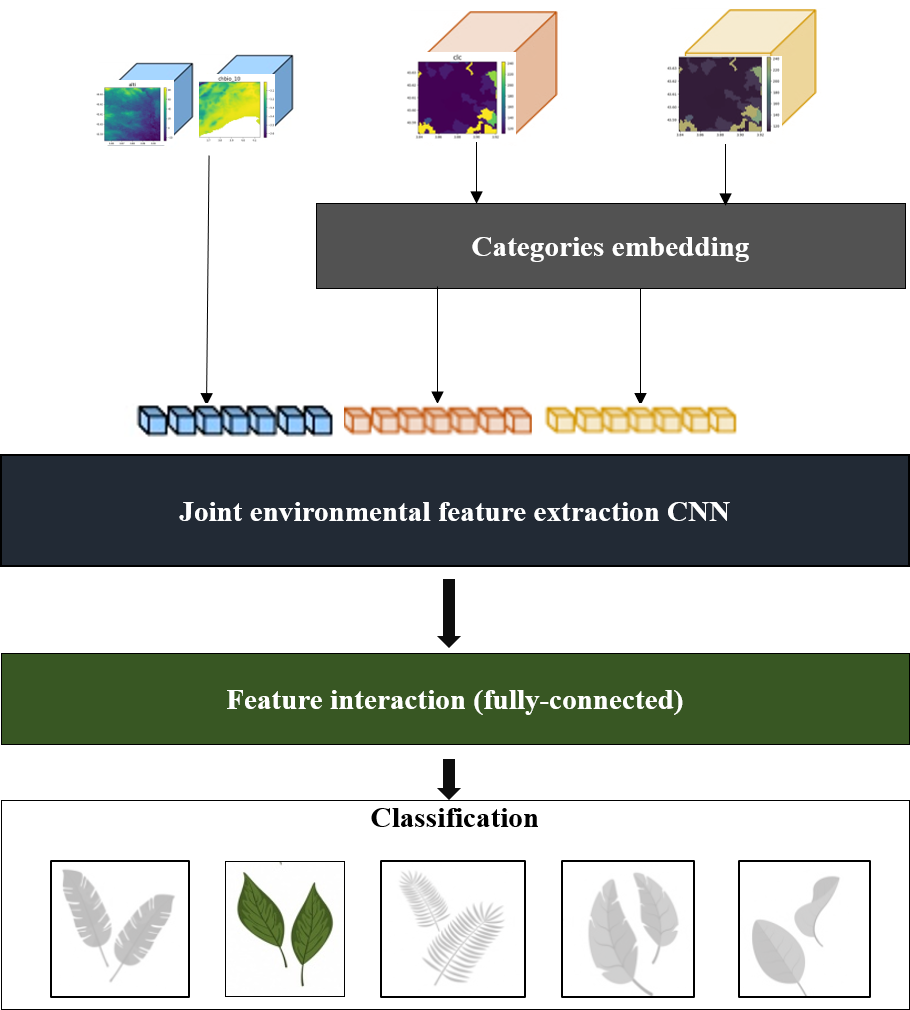
\includegraphics[scale=0.4]{grinnelljoint.png}
		\caption{JointGrinnellNet: joint feature extraction} \label{grinnellnet:b}
	\end{subfigure}
	\caption{GrinnellNet architecture} \label{grinnellnet}
\end{figure}

\subsubsection{Input preprocessing}
%\paragraph{Ecological motivation for spatial input}\mbox{}\\
%Why we use patches instead of simply extracting values in given locations%
%Observed location is not necessarily optimal habitat%
Observing a species in a given location does not necessarily imply a suitability of the abiotic environment. Indeed, some species survive in locations with unfavorable conditions (sink) as long as new individuals continuously join the population from a nearby suitable habitat (source), through seed dispersal for instance via wind currents. These so called source-sink dynamics \cite{holt1985population} ensure an indefinite sustainability of the sink populations despite unfavorable abiotic conditions. %In other locations with similar abiotic conditions, the species may not be observed if there is no accessible favorable habitat or source population. %
Consequently, failing to account for these spatial processes may result in overestimation of the species environmental niche's breadth.
%GPS uncertainty%
Beyond stochastic assembly processes, geographic coordinates measured by various smartphone devices present an uncertainty that needs to be accounted for.\\\\
%Why we use CNNs to process patches: end-to-end feature extraction with accounting of spatial structure%
\noindent For the previous reasons, it is necessary to consider a landscapewise rather than a pointwise description of the environment around the observation geolocation by using environmental patches instead of local values.\\ 

\noindent We group the environmental rasters into three groups based on their semantic, the resolution at which they vary and their data type (quantitative, ordinal and categorical). 

\begin{itemize}
	\item \textbf{TopoHydroClimate} group: quantitative variables describing global bioclimate (CHBIO, ETP), hydrology (water proximity) and topology (altitude).
	\item \textbf{Pedology} group: ordinal and categorical variables describing the physico-chemical structure of the soil.
	\item \textbf{Land use} group: includes corine land cover class. 
\end{itemize}

%We apply the following specific treatments for categorical and some ordinal variables with small cardinality:

\paragraph{Embedding categorical features}\mbox{}\\
Part of the soil physico-chemical properties are described by categorical or pseudo-ordinal features such as texture, land cover, erodibility and crusting class. Therefore, for each categorical feature $F_c$, before feeding it to the CNN layers, we replace each of its $N_c$ categories by a real vector representation of size $K_c$. In practice, this is implemented by a feature-specific embedding lookup layer parameterized by a $(N_c,F_c)$ matrix $E_c$, such that $E_c[i,]$ is the $K_c$ sized embedding of the $i^{th}$ value of $F_c$. We apply this transformation batchwise in parallel to all patch cells. For an input of dimension $(BatchSize, PatchRadius, PatchRadius, 1)$, the embedding layer of $F_c$ returns a tensor of dimension $(BatchSize, PatchRadius, PatchRadius, K_c)$. These vector representations are trained along with other network parameters whereas $K_c$ is a tunable hyperparameter, typically chosen in the interval $[\![2,\frac{N_c}{2}]\!]$. \\

\noindent Categorical embeddings capture richer relationships than raw categories. They are also considered as a dimensionality reduction technique, more practical than one-hot-encoding when dealing with high-cardinality yet sparse features (a typical example in our case is land cover). Note that each embedding dimension could have multiple meanings that do not necessarily line up with ordinal dimensions. In the end, categories with similar representations translate a similar effect on the target variable.\\

\paragraph{Resulting preprocessed inputs}\mbox{}\\
\noindent Pedological features embeddings resulting from the previous step are concatenated into a single tensor of dimension:\\ $(BatchSize, PatchRadius, PatchRadius,\sum_{c \in C}{K_c}=18)$, such that $C$ refers to the set of categorical features. Land cover is embedded separately.\\

\noindent Climate, topological and hydrological features are input to the neural network as batches of multi-channel images of dimension equal to $(BatchSize, PatchRadius, PatchRadius, N_{num})$, $N_{num}=22$ being the number of features.

\subsubsection{Feature extraction}
We investigated two modes of feature extraction on the preprocessed inputs:
\begin{itemize}
	\item \textbf{JointGrinnellNet}: A joint mode where all input tensors are concatenated into a single multi-channel image of size: $(BatchSize, PatchRadius, PatchRadius, \sum_{c \in C}{K_c} + N_{num})$. The result is fed into a feature extraction module, presented in Figure \ref{grinnellnet:a}.
	\item \textbf{SepGrinnellNet}: A separate mode where the three groups of features are treated separately by dedicated feature extraction modules then merged afterwards, presented in Figure \ref{grinnellnet:b}.
\end{itemize} 

%\paragraph{Feature extraction module architecture}\mbox{}\\
\noindent Spatial data use requires appropriate feature extraction techniques that are able to harness the spatial structure of such inputs. Convolutional neural networks\cite{lecun1995convolutional}, a class of artificial neural networks inspired from the virtual cortex of animals, constitute an ideal choice as they allow to extract features from spatially-structured inputs within an end-to-end learning process. They have been previously shown to provide substantial improvements in predicting species abundance \cite{botella2018deep,deneu2018location}.\\

\noindent Each of our CNN-based feature extraction modules comprise a 2-block architecture similar to VGG\cite{simonyan2014very}. Each block contains two 3x3 convolution layers set to extract 256 features, followed by MaxPooling then a Leaky Rectified Linear Unit activation. The latter function choice prevents the model from falling into a dying ReLu problem (experienced during first tests with ReLu activation)\cite{maas2013rectifier}. Retained embedding sizes, patch radius and resulting number of channels are shown in the detailed architecture (see Appendix).

\subsubsection{Feature interaction and classification components}
Extracted features from the different components are flattened and eventually concatenated into a single large vector. This vector is then fed into a fully connected neural network dedicated to learning the separation of the plant classes in the learnt feature space. This feature interaction component comprises 3 dense layers of respectively 8192, 4096 and 3353 neurons. We applied a 0.75 dropout rate on the intermediary layers to prevent overfitting. The classification layer consists on a softmax activation applied on the output to determine the probabilities of each class. Class probabilities sum to 1 by definition. Naturally, the one with the highest probability is attributed to the instance. 

\subsection{EltonNet: a species embedding network}
Here we propose to rely purely on plant associations to other taxonomic groups. The goal is to predict the dominant plant from knowledge of the occurrences of other taxa around it, up to a certain radius. In order to reduce the number of co-occurring organisms, address the rarity of some of them and capture stronger associations with plants, the following steps were applied to non plant occurrences. 

\subsubsection{Taxonomic grouping and biogeographical filtering}
We aggregated taxa according to ecological knowledge on the taxonomic level where biogeographical correlations to plants are meaningful. This level differs from one group to another, thus different preprocessing schemes were applied to different taxonomic groups. Then, for some groups we used domain-knowledge heuristics to filter irrelevant groups. Proportions of retained groups in the taxa list are illustrated in Figure \ref{proponp}. Finally, we assigned internal codes, unique identifiers, to each group. 

\paragraph{Fungi selection}
We grouped fungal species by genus. Then, we used FunGUILD database\cite{nguyen2016funguild} to select fungi from guilds (groups with similar diets and functions in the ecosystem) that are dependent on plants for feeding. We kept the following guilds: Pathotrophs (parasites of plants) and Symbiotrophs (involved in positive associations with plants such as mycchorizea). We deleted Saprotrophs (organic matter decomposers) as they do not depend on plants whatsoever. In the end, we retained 195 out of 531 genuses. 

\paragraph{Insects selection} 
We aggregated insects to the order level except for Coleoptera and Orthoptera which were grouped in families as they exhibit significant intraorder variability in terms of habitat preferences and diet. We chose among insect orders those with known co-evolution history with plants (such as Hymenoptera) and/or established potential for direct interaction with plants (such as pollinators and herbivores)\cite{sauvion2013interactions}. The intuition is that some insects have strong affinities or preferences (such as specialist pollinators) towards specific plants which leads to a greater chance of co-existence. This process led to the selection of 464 families of Coleoptera and Orthoptera in addition to 9 other orders.  

\paragraph{Aves selection}
Most birds breed in their preferential habitat during the period spanning from March to July. The rest of the year, during their migration phase, they pass by other areas where they can be occasionally observed. We considered these observations as spurious and removed them to avoid establishing false associations to plants. We then aggregated birds to the genus level. Afterwards, we used www.oiseaux.net to identify and remove some introduced/invasive genuses.  We ended up with 240 bird taxa. 
%(Acridotheres, Aegypius ,Agapornis, Aix, Alcedo, Alle, Alopochen)

\paragraph{Amphibians, mammals and reptiles aggregation} 
Lacking expert knowledge on these phyla, we simply grouped them to the genus level, yielding respectively 21 amphibians, 93 mammals, and 33 reptiles.

\begin{figure}[h]
	\centering
	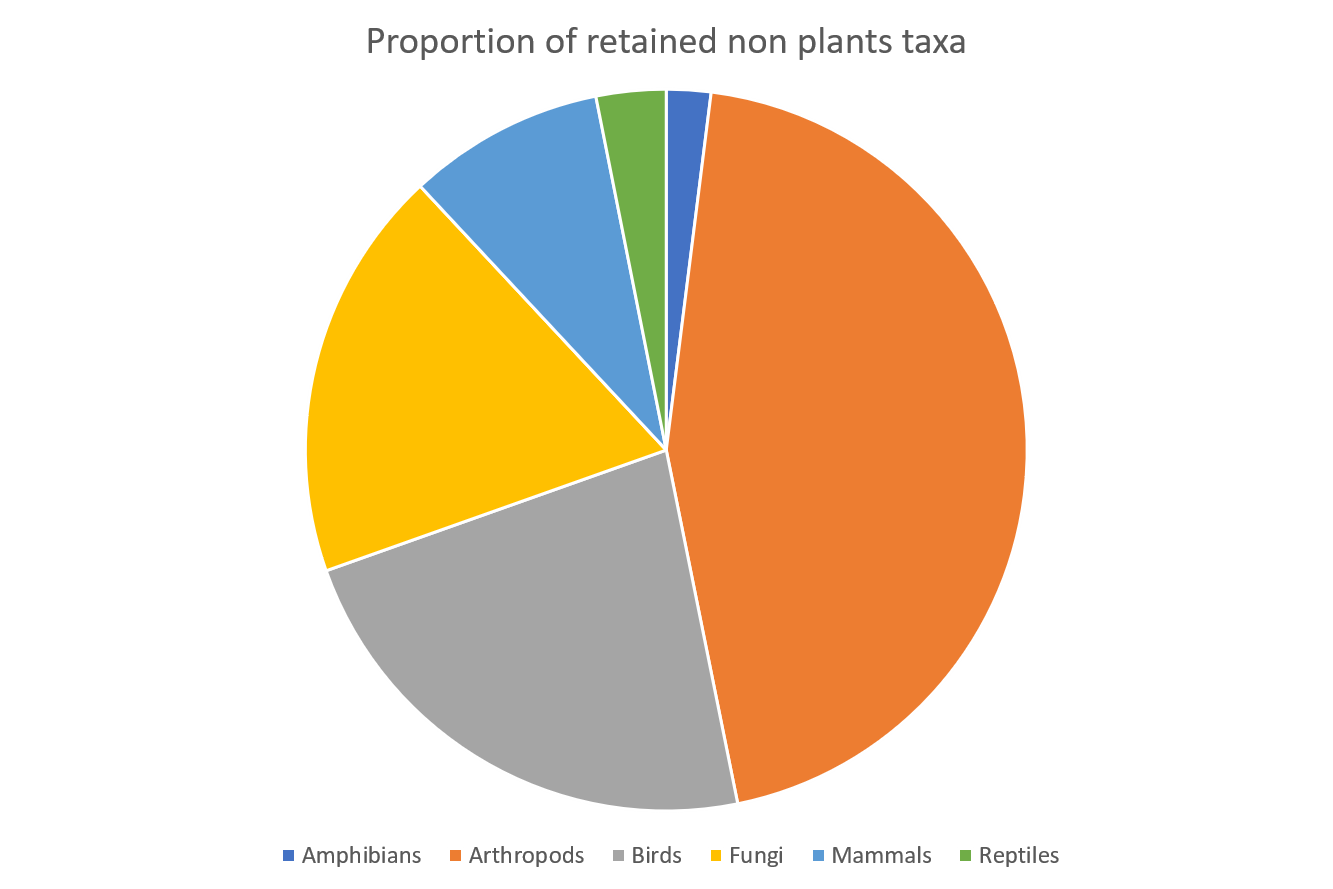
\includegraphics[scale=0.5]{proportion}
	\caption{Non plants taxa proportion in the retained list.}
	\label{proponp}
\end{figure}

\subsubsection{Biotic context calculation}
To accelerate the training phase, we precomputed for each training example $i$, given its coordinates, the set $NP_i$ of non plant observations that occur at a maximum radius of 8 Km. We started with 500m then we doubled the radius each time the search of neighbors yielded an empty set. We stopped when we reached 8 Km. Afterwards, we randomly draw with repetition $W$ observations from $NP_i$ with a uniform probability. That way, more abundant taxa (present multiple times in $NP_i$) have a higher probability of being included. At the end of this process, we had associated each training example to its biotic context made of $W$ observations of organisms from other kingdoms.   

\subsubsection{The species embedding network architecture}
The learning model used is a customized keras implementation of the Continuous Bag of Words model first introduced in \cite{mikolov2013efficient}. The architecture, illustrated in Figure \ref{eltonnet}, is based on a neural network composed of 3 layers:\\

\noindent- The input layer of size $W$ receives the identifiers of the biotic context components.\\
- An embedding layer that associates a real-valued vector of size $K_{np}$ for each taxa (non plants). This embedding vector captures the effect of observing this organism on the odds of each plant class. \\
- A lambda averaging layer that aggregates the biotic context embeddings. \\
- A dense layer that computes for each target plant species the dot products of its weight vector to the aggregated context embedding. This layer uses a softmax activation to return the probabilities of each target plant to occur given the observations of the surrounding non plants. \\

\begin{figure}[h]
	\centering
	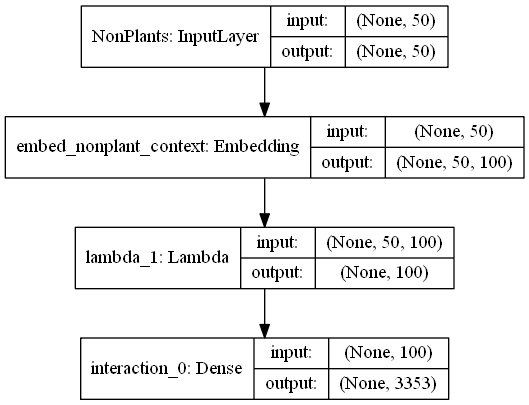
\includegraphics[scale=0.3]{elton}
	\caption{EltonNet architecture}
	\label{eltonnet}
\end{figure}

\section{Training end evaluation}
\subsection{Optimization and evaluation metrics}
For both proposals, we optimize the class-weighted sparse categorical crossentropy loss given by equation Eq \ref{softmax}. Given:\\
- $ P $: the set of plant classes (here species-level identifications).\\
- $ p $: the expected or true class.\\
- $s_p$: the neural network output probability for the true class.\\
- $w_p$: weight of the true class.

\begin{gather}
CE = - w_p log(\dfrac{\exp^{s_p}}{\sum_{j}^{P} \exp^{s_j}})
\label{softmax}
\end{gather}

\noindent Some species were observed more often than others (see Figure \ref{classcardinality}), which created a class-imbalance problem within the training set. To address this issue, we weighted each training example by the weight of its expected class (see Eq \ref{cweight}). This strategy allowed us to give more importance to the misclassification of rare classes observations (correcting for false negatives).  Each class c with a prevalence $p_c$ on the training set was attributed a weight computed as the ratio of its points of absence to its points of presence. 
\begin{gather}
w_c = \frac{1-p_c}{p_c}
\label{cweight}
\end{gather}  

\noindent This process is particularly useful for endemic species of undersampled locations.   

\begin{figure}[h]
	\centering
	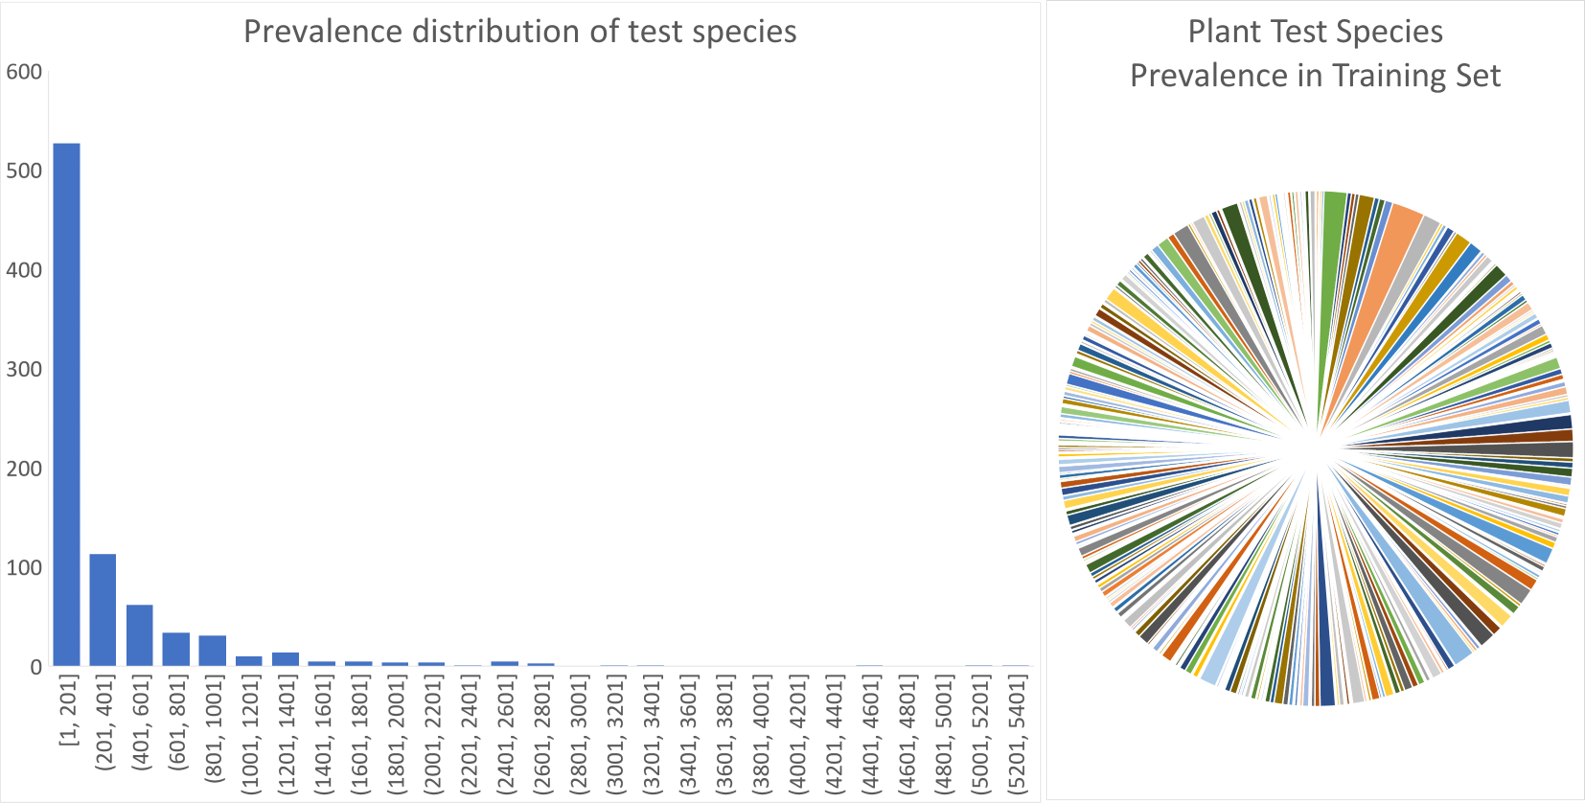
\includegraphics[scale=0.5]{classcardinality}
	\caption{Species prevalence distribution in the full training dataset: statistics are computed on plants included in the test set only.}
	\label{classcardinality}
\end{figure}

\subsection{Implementation and learning setting}
\noindent We implemented GrinnellNet and EltonNet in Python\footnote{https://www.python.org/} using Keras deep learning framework with Tensorflow\footnote{https://www.tensorflow.org/guide/keras} backend. We trained the models using multigpu data parallelism on a single computing node equiped with 4 GPUS V100 with NVlink. We used adam\cite{kingma2014adam} optimization algorithm with a decaying learning rate starting from 0.001 and reduced by a 10 factor whenever the validation loss stops improving after 5 epochs. \\ 

\subsection{Evaluation}
\noindent We sampled 80\% of the dataset for training and kept the remaining 20\% for validation. We used a stratified cross-validation split procedure to ensure coverage of all classes in the training set. At the end of every epoch, we evaluated the prediction accuracy of the models on the validation set. Figure \ref{perfs} summarizes the performances obtained during training (left axis) along with results on test set (right axis). Note that different evaluation metrics are used. As a result, we can only compare the models ranking.\\

\noindent ELT100 and ELT300 correspond to EltonNet applied to occurrences of test species (evaluated in the test set) with an embedding size  $K_{np}$ taking respectively the values $100$ and $300$.  GRIN\_SEP and GRIN\_SEP+ (trained longer) apply GrinnellNet on occurrences of all plant species whereas in GRIN\_SEP\_TEST the model is trained only on test species. GRIN\_SEP uses separate feature extraction components for each feature group while GRIN\_JOINT uses the joint feature extraction mode. 

\begin{figure}[h]
	\centering
	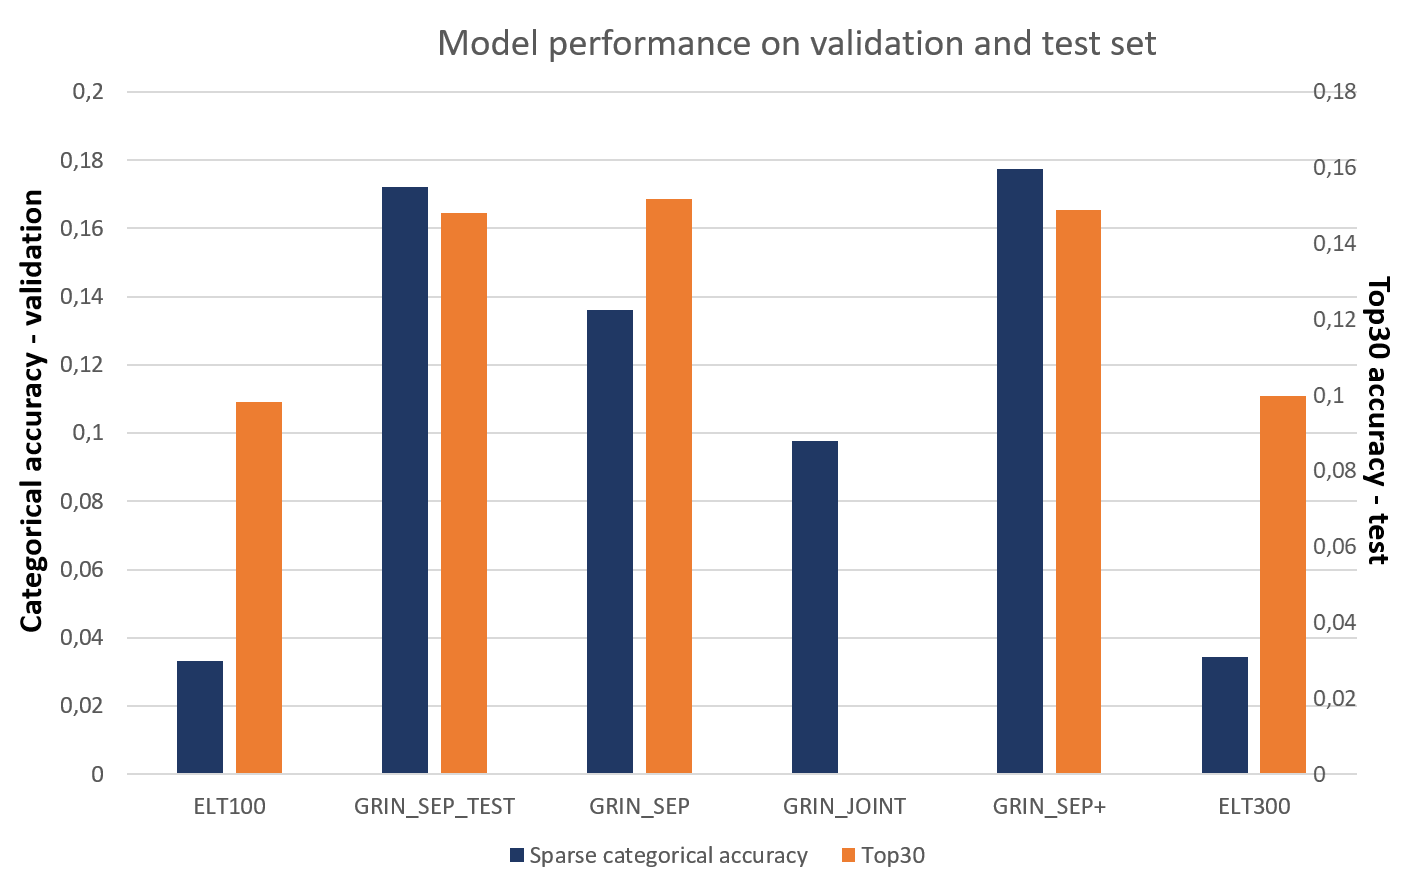
\includegraphics[scale=0.7]{trainingperfs}
	\caption{Performance of GrinnellNet and EltonNet variants on validation and test set.}
	\label{perfs}
\end{figure}

\noindent Unsurprisingly, GrinnellNet performs much better than EltonNet. Indeed, we would expect such results as covariates used in the former are richer and unbiased. Besides, biogeographical theory recognizes the superiority of the abiotic filter in selecting species\cite{boulangeat2012accounting}, as it is directly related to their physiological traits. On the other hand, EltonNet resulted from a series of arbitrary domain heuristics. Nevertheless, it still performs better than random with relatively strong associations learnt between plants and other taxa, an unneglectable insight for community ecologists.\\

\noindent In the case of GrinnellNet, the choice of the feature extraction mode clearly affects its predictive performances. Results show that treating the feature groups separately leads to better performances. This can be explained by the nature of the data encoded in the rasters that were created/interpolated from different data collection protocols. Indeed, pedological characteristics for instance are mainly determined by subjective field observations whereas climate data are calculated with advanced mathematical models. Another possible reason to separate the feature extraction processes is the scale at which the rasters were constructed. While, bioclimatic variables are interpolated to the kilometer in regular grids, soil data are aggregated using anthropo-topological polygons to the landscape level, which translates in several kilometers. Consequently, we only submitted GRIN\_SEP runs for the task.\\

\noindent We also observed that better performances on the validation set were obtained with weighting strategies compared to no correction of class-imbalance (not shown here). Furthermore, the runs ranking on the validation set is roughly the same as in the test set results except for GRIN\_SEP and GRIN\_SEP\_TEST. During validation, we found that GrinnellNet performs better when it is trained solely on test species than when it uses occurrences of all plant species. At test time, the order was reversed which might be a sign of overfitting in GRIN\_SEP. But also, because GRIN\_SEP\_TEST is exposed to more observations it probably learns more robust features.
 

\section{Conclusion}
We presented two proposals for the location-based species recommendation problem. The first solution leverages the concept of Grinnellian niche by basing its predictions on only abiotic features, automatically extracted from environmental rasters using convolutional neural networks. This approach can be extended to any taxonomic group beyond plants. Moreover, we investigated the use of distributed representations as a means to reduce feature dimensionality as well to capture rich semantic associations. \\ 

\noindent In the second proposal, we attempted to learn the Eltonian niche of the plants by embedding the biotic contexts where they're observed. We relied heavily on domain knowledge with expert assistance to filter co-occurrences in order to learn strong associations. Although the assumptions and rules used to select non plants species were specific to plant modeling, the learning architecture itself can be used for any taxonomic group. Additionally, this approach suffered from heterogeneous sampling effort. Ideally, one could use projection maps predicted by species distribution models when available as input to a convolutional neural network.\\ 

\noindent The global result is that the CNN solution outperformed the species embedding approach. But the latter allowed us to identify associations between plants and other taxa which can be used to develop bioindicators. In the end, one could train both models jointly with shared layers that can capture the interactions and possible feedbacks between biotic and abiotic variables.
  
\bibliographystyle{acm}
\bibliography{biblio/hsmbiblio}	

\appendix
\begin{figure}
	\centering
	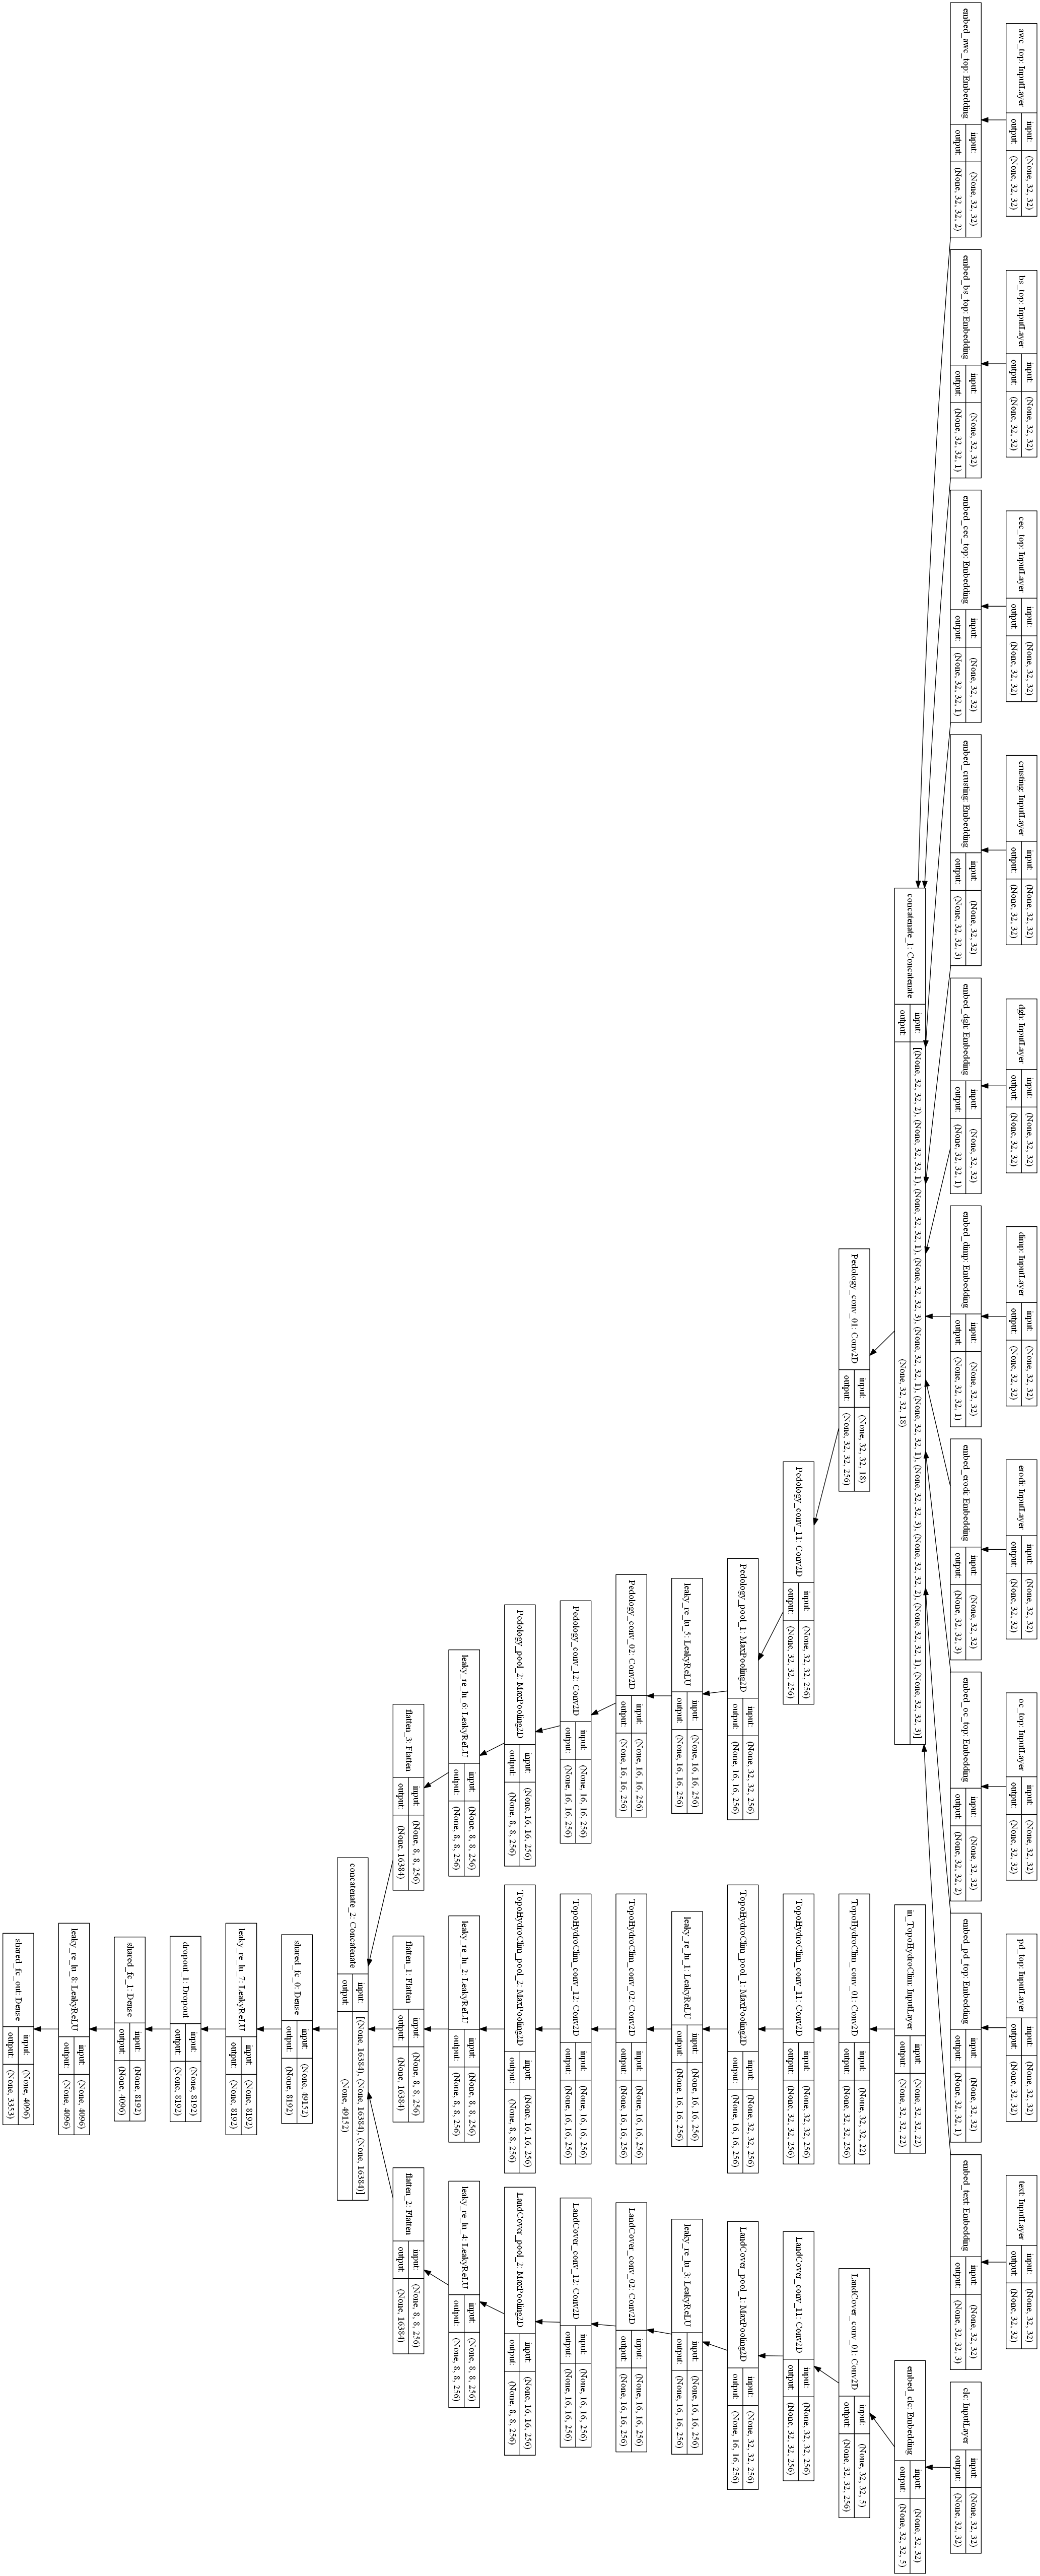
\includegraphics[scale=0.15]{grinnell}
	\caption{GrinnellNet architecture: separate feature extraction components.}
	\label{grinnarchi}
\end{figure}
\end{document}
